% Подписи колонтитула
\newcommand{\colontitulAutors}{edombek, astronom\_v\_cube et al.}
\newcommand{\colontitulYear}{2022}
\newcommand{\colontitulEducationalSubject}{Прикладная электродинамика}
\newcommand{\colontitulTeacher}{Гиндельбург~В.~Б.}

%Настройки шаблона
\documentclass[10pt,landscape,a4paper]{article}
\usepackage[utf8]{inputenc}
\usepackage[english, russian]{babel}
\usepackage[T1,T2A]{fontenc}  
\usepackage{upgreek} % прямые греческие ради русской традиции
\usepackage{tikz}
\usetikzlibrary{shapes,positioning,arrows,fit,calc,graphs,graphs.standard}
%\usepackage[nosf]{kpfonts}
%\usepackage[t1]{sourcesanspro}
\usepackage{multicol}
\usepackage{wrapfig}
\usepackage[top=6mm,bottom=8mm,left=4mm,right=4mm]{geometry}
\usepackage[framemethod=tikz]{mdframed}
\usepackage{microtype}
\usepackage{pdfpages}
\usepackage{amsthm,amsmath,amscd}   % Математические дополнения от AMS
\usepackage{amsfonts,amssymb}       % Математические дополнения от AMS
\usepackage{mathtools}              % Добавляет окружение multlined
\usepackage{xfrac}                  % Красивые дроби
\usepackage{physics}

\usepackage{fancyhdr} % колонтитулы

%некоторые математические команды
\newcommand{\Div}{\operatorname{div}}
\newcommand{\Grad}{\operatorname{grad}}

\let\bar\overline

\definecolor{myblue}{cmyk}{1,.72,0,.38}

\def\firstcircle{(0,0) circle (1.5cm)}
\def\secondcircle{(0:2cm) circle (1.5cm)}

\colorlet{circle edge}{myblue}
\colorlet{circle area}{myblue!5}

\tikzset{filled/.style={fill=circle area, draw=circle edge, thick},
	outline/.style={draw=circle edge, thick}}

\pgfdeclarelayer{background}
\pgfsetlayers{background,main}

%\everymath\expandafter{\the\everymath \color{myblue}}
\everydisplay\expandafter{\the\everydisplay \color{myblue}}

\renewcommand{\baselinestretch}{.8}
\pagestyle{empty}

\global\mdfdefinestyle{header}{%
	linecolor=gray,linewidth=1pt,%
	leftmargin=0mm,rightmargin=0mm,skipbelow=0mm,skipabove=0mm,
}

\makeatletter % Author: ttps://tex.stackexchange.com/questions/218587/how-to-set-one-header-for-each-page-using-multicols
\renewcommand{\section}{\@startsection{section}{1}{0mm}%
	{.2ex}%
	{.2ex}%x
	{\color{myblue}\sffamily\small\bfseries}}
\renewcommand{\subsection}{\@startsection{subsection}{1}{0mm}%
	{.2ex}%
	{.2ex}%x
	{\sffamily\bfseries}}

\makeatother
\setlength{\parindent}{0pt}

%колонтитулы
\pagestyle{fancy}
\fancyhf{}
\setlength{\headheight}{40pt}
\setlength{\headsep}{4pt}
\renewcommand{\headrulewidth}{1pt}
\fancyhead[L]{\textcopyright~\colontitulAutors}
\fancyhead[C]{Программа минимум по курсу <<\colontitulEducationalSubject>> \colontitulYear г}
\fancyhead[R]{Преподаватель:~\colontitulTeacher}

\renewcommand{\frac}{\dfrac} % большие дроби
\newcommand{\eps}{\varepsilon}

\begin{document}
	\small
	\begin{multicols*}{2}
		\section{Запись функции, определяющей зависимость полей и векторных потенциалов гармонической плоской волны в линии передачи от времени $t$ и продольной координаты $z$. Понятия частоты, временного периода, продольного волнового числа, длины волны, фазовой и групповой скорости.}
		$\{\vec{E},\vec{H}\}=\{\vec{E_0},\vec{H_0}\}e^{i(wt-hz)}, ~\vec{A}^{e,m}=\vec{z_0}\psi^{e,m}(r_{\perp})e^{-ihz}$ \\
		$\psi$~-~произвольная скалярная функция(амплитуда векторного потенциала), $(wt-hz)$~-~фаза \\
		$\varkappa^2=k^2-h^2$~-~поперечное волновое число, $k=\frac wc\sqrt{\mu\eps}$~-~волновое число в среде, $ h $~-~ продольное волновое число. \\
		$T=\frac {2\pi}w, \lambda_\text{в}=\frac {2\pi}h, V_\text{ф}=\frac{w}{h}, V_\text{гр}=\dv{w}{h}$. Для волновода без заполнения $V_\text{ф}V_\text{гр}=c^2$. $V_\text{гр}\le c$.
		
		\section{Волновое уравнение для векторного потенциала в отсутствие источников при произвольной и гармонической зависимости от времени. Дифференциальное уравнение для скалярных поперечных волновых функций $\Psi^{(e),(m)}(r_\perp)$, определяющих зависимость полей в линии передачи от поперечных координат. Понятие поперечного волнового числа. }
		
		$\Delta \vec{A}-k^2\vec{A}=0, \Delta=\frac{\partial^2}{\partial z^2}+\Delta_\perp, \Delta_\perp=\frac{\partial^2}{\partial x^2}+\frac{\partial^2}{\partial y^2}, \frac{\partial^2}{\partial z^2}=-h^2$. \\
		При гармонической зависимости от $t$: $\Delta \vec{A_\perp}-(k^2-h^2)\vec{A}=0$.\\
		Решение: $\vec{a}^{e,m}=\vec{z_0}\psi^{e,m}(r_\perp)e^{-ihz}$ (в отсутствии сторонних источников); \\
		TE($ E_z=0 $): $ \Delta_\perp\psi^m+\varkappa^2\psi^m=0 $; \\
		TM($ H_z=0 $): $ \Delta_\perp\psi^e+\varkappa^2\psi^e=0 $; \\
		TEM($ E_z=0 $): $ \Delta_\perp\psi=0 $.\\
		$\varkappa^2=k^2-h^2$~-~поперечное волновое число. \\
		
		$\varkappa_n=\sqrt{\frac{w^2}{c^2}\mu\eps+h_n^2}, \quad n=0,1,2,...$~-~номер моды.
		
		\section{Понятие о ТЕ, ТМ и ТЕМ волнах. Импедансная связь поперечных компонент полей. Определение поперечного волнового импеданса. }
		
		$\{\vec{H},\vec{E}\}=\vec{z_0}\{{H_z},{E_z}\}+\{\vec{H_\perp},\vec{E_\perp}\}$ \\
		\begin{tabular}{l l l}
			TM($H_z=0$) & TE($E_z=0$) & TEM($E_z=H_z=0$) \\
			$\begin{rcases}
				E_z=\frac{\varkappa^2}{ik_0\eps\mu}\psi^e \\
				\vec{E_\perp} = \frac{-h}{k_0\eps\mu}\nabla_\perp\psi^e \\
				\vec{H_\perp}=\frac1{\mu}[\nabla_\perp\psi^e,\vec{z_0}]
			\end{rcases} e^{i(wt-hz)}$ & 
			$\begin{rcases}
				H_z=\frac{\varkappa^2}{ik_0\eps\mu}\psi^m \\
				\vec{H_\perp} = \frac{-h}{k_0\eps\mu}\nabla_\perp\psi^m \\
				\vec{E_\perp}=\frac1{\eps}[\nabla_\perp\psi^m,\vec{z_0}]
			\end{rcases} e^{i(wt-hz)}$ & 
			$\begin{rcases}
				\vec{E_\perp} =-\frac1{\sqrt{\eps\mu}}\nabla_\perp\psi \\
				\vec{H_\perp}=\frac1{\mu}[\nabla_\perp\psi,\vec{z_0}]
			\end{rcases} e^{i(wt-hz)}$ \\
		\end{tabular}
		$E_\perp=\zeta_\perp[\vec{H_\perp},\vec{z_0}]$~-~импедансная связь \\
		Поперечный импеданс($\zeta_\perp$): \\
		\begin{tabular}{l l l}
			TE & TM & TEM \\
			$\sqrt{\frac{\mu}{\eps}}\frac kh$ & $\sqrt{\frac{\mu}{\eps}}\frac hk$ & $\sqrt{\frac{\mu}{\eps}}$ \\
		\end{tabular}
		
		\section{Граничные условия для полей и поперечных волновых функций $\Psi^{(e)}$ и $\Psi^{(m)}$ в линиях передачи с идеально проводящими границами. Математическая формулировка задачи отыскания собственных волн различных типов в идеальной линии.}
		
		$E_\tau=0, H_n=0$ - Г.~У. \\
		\begin{tabular}{l l l}
			TE: & TM: & TEM: \\
			$\begin{cases}
				\Delta_\perp\psi^m+\varkappa^2\psi^m=0 \\
				\pdv{\psi^m}{n}|_{L}=0 \text{~-~условие Дирихле}\\
			\end{cases}$  &
			$\begin{cases}
				\Delta_\perp\psi^e+\varkappa^2\psi^e=0 \\
				\pdv{\psi^e}{n}|_{L}=0 \text{~-~условие Неймана}\\
			\end{cases}$  &
			$\begin{cases}
				\Delta_\perp\psi=0 \\
				\psi=const_i|_{L_i}\\
			\end{cases}$ \\
		\end{tabular}
		
		\section{Дисперсионное уравнение для волн в идеальных линиях. Понятие критической частоты и критической длины волны. Графики зависимости полей от продольной координаты в различные моменты времени при частотах, больших или меньших критической. Зависимости длины волны, фазовой и групповой скорости в линии передачи от частоты.}
		
		$h_n = \pm \sqrt{k^2 - \varkappa^2} = \pm \sqrt{\dfrac{\omega^2 \varepsilon \mu}{c^2} - \varkappa_n^2}$, \quad $n = 1,~2,~3...$ - номер моды\\
		В ИЛП есть бесконечные наборы $ТЕ$ и $ТМ$ волн, называемые модой. Любой моде соответствует своё дисперсионное соотношение. При этом $\varkappa_n$ не зависит от $\omega,~\varepsilon,~\mu$, а определяется геометрией ЛП.\\
		Существует критическая частота, при которой осуществляется переход от распространения волны ($\varepsilon > \varepsilon_\text{кр}$) к нераспространению ($\varepsilon < \varepsilon_\text{кр}$).\\
		$\omega_\text{кр n} = \dfrac{\varkappa_n c}{\sqrt{\varepsilon \mu}}$; \quad $\lambda_\text{кр n} = \dfrac{2\pi \varepsilon \mu}{\varkappa_n}$\\
		
		\begin{tabular}{l l}
			{Распространение} & {Нераспространение} \\
			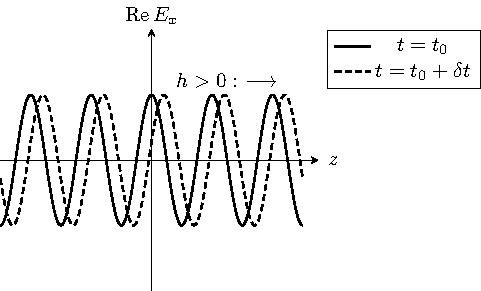
\includegraphics[width=0.25\linewidth]{aed_imgs/lect3_ris1} &
			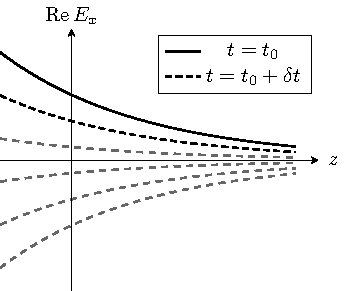
\includegraphics[width=0.25\linewidth]{aed_imgs/lect3_ris2} \\
		\end{tabular}
		
		\section{В каких линиях могут существовать главные (ТЕМ) волны? Поля ТЕМ волны в коаксиальной линии (форма силовых линий и зависимость от координат).}
		
		TEM-волна~--~волна, где присутствуют только поперечные компоненты полей ($E_z = H_z = 0) \Rightarrow h = k$,~ $\varkappa = 0$. Предположим, что в волноводе распространяется волна, у которой векторы $\vec{E}$ и $\vec{H}$ лежат в поперечной плоскости. Силовые линии вектора $\vec{H}$, являясь замкнутыми, должны охватывать линии тока. Но токи проводимости отсутствуют, поскольку внутри волновода проводников нет. Значит, током может быть только продольный ток смещения. Поэтому должна иметься продольная составляющая вектора. Следовательно, ТЕМ-волна (волна без продольной составляющей вектора) в волноводе не может распространяться. Из этих рассуждений ясно, что для существования ТЕМ-волны в замкнутой направляющей системе необходимо, чтобы последняя состояла \textbf{не менее чем из двух изолированных друг от друга проводников}, по которым может протекать ток проводимости (коаксиальная линия, полосковая и пр.)\\
		\begin{tabular}{l}
			{Поле в коаксиальном кабеле} \\
			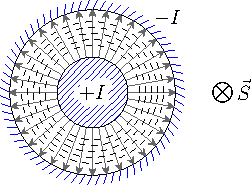
\includegraphics[width=0.25\linewidth]{aed_imgs/lect4_ris6} \\
		\end{tabular}
		
		\section{Спектр поперечных волновых чисел прямоугольного волновода. Низшая мода (поперечное волновое число, графики поля, картина силовых линий). Низшая мода круглого волновода (поперечное волновое число, картина силовых линий).}
		
		\section{Причины затухания волн в линиях передачи. Описание затухания, обусловленного потерями энергии в заполняющей среде. Графики зависимости поля в линии передачи с потерями от продольной координаты в различные моменты времени.}
		
		\section{Описание главных волн в линиях передачи в терминах тока и напряжения: определения величин тока и напряжения, погонной емкости и индуктивности, определения волнового сопротивления, импеданса нагрузки, импеданса в любом сечении линии с произвольной нагрузкой на конце.}
		
		\section{Коэффициент отражения волны от нагрузки на конце линии. Понятие согласования линии с нагрузкой.}
		
		\section{Спектр собственных частот идеального прямоугольного резонатора. Низшая мода прямоугольного резонатора (собственная частота, структура поля).}
		
		\section{Причины затухания колебаний в реальных резонаторах. Описание затухания, обусловленного потерями энергии в заполняющей среде. График зависимости поля собственного колебания в реальном резонаторе от времени.}
		
		\section{Представление полей, создаваемых в волноводе заданными сторонними токами, в виде суперпозиции полей собственных мод (общий вид формул возбуждения волноводов).}
		
		\section{Представление полей, создаваемых в резонаторе заданными сторонними токами, в виде суперпозиции полей собственных колебаний (общий вид формул возбуждения резонатора). Резонансные свойства полей. }
		
		\section{Способы возбуждения волноводов и резонаторов при помощи штыря и петли.}
		
		\section{Определения дифференциального и полного сечений рассеяния тела. Выражение для амплитуды поля и плотности потока энергии рассеянной волны в дальней зоне через дифференциальное сечение рассеяния. }
		
		\section{Приближение геометрической оптики и условия его применимости в задачах дифракции плоской волны на теле. Понятие луча и лучевой трубки. }
		
	\end{multicols*}
\end{document}